\chapter{Introduction}
\label{introduction}

\section{Message Domain/Signal Domain}

\section{What is aliasing?}
Aliasing in audio means problems caused by signals that exceed the nyquist rate.\\
The nyquist rate,let's call it $f_n$ for now, is defined by the half of the sample rate ($f_s$). So, 
\begin{equation}
	f_n=\frac{f_s}{2}
\end{equation}
A digital system can only describe signals up to his nyquist rate. If we try to make signals higher than this frequency, we will fail and encounter strange effects.\\
Visually speaking, frequencies higher than nyquist fold back. So, let's assume we have a sampling rate of 100Hz. Nyquist would be at 50Hz. If we try to synthesize a sine wave with 51Hz, what we will get is a 49Hz one. If we try to make a 52Hz one, we will get 48Hz. So you see, it simply folds back.



\section{Scaling and Mapping Signals}
It is an important skill to be able to scale signals from one range to another. We need it a lot and we will be able to think about signals more easily f we mastered this task. It's actually quite simple, we just have to imagine the signals visually.\\
So what exactly do we have to do here? We are confronted with the following problem: Given some signal, say, a sine wave with its maximum at the value 1 and its minimum at the value -1. How to bring it to a different range, say, 0-10?\\
It helps me a lot to solve this problem in two parts: first get the input in the range 0-1, then from there go to the desired range. What can we do to the signal? Let's take a sine wave:

\begin{figure}[h!]
	\centering
	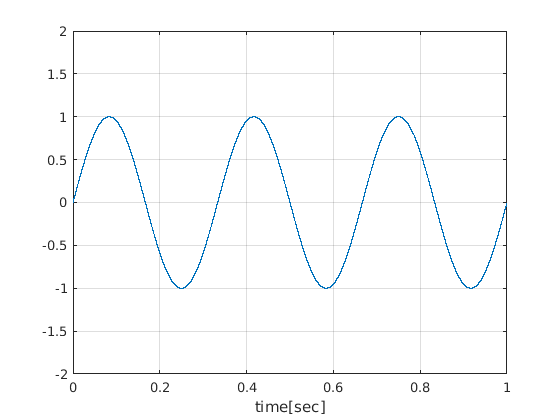
\includegraphics[width=11cm]{stdSine.png}
	\caption[a sine wave]
	{a sine wave}
	\label{fig:aSine}
\end{figure}
Well we can add and subtract to move the wave vertically, so let's add 1 to move it up:

\begin{figure}[h!]
	\centering
	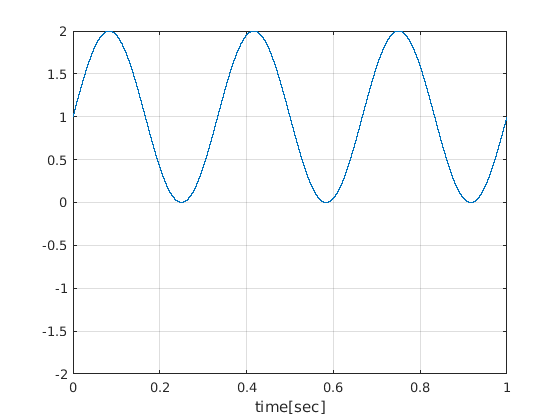
\includegraphics[width=11cm]{sinePlusOne.png}
	\caption[a sine wave]
	{the same sine wave, 1 added to a each sample, therefore shifted upwards.}
	\label{fig:aShiftedSine}
\end{figure}

So we can move signals around by adding constant values. We can scale them by multiplication. So if we take our sine that now ranges from 0 to 2 and multiply it by 0.5, we get whats in figure \ref{fig:sine01}.

\begin{figure}[h!]
 	\centering
 	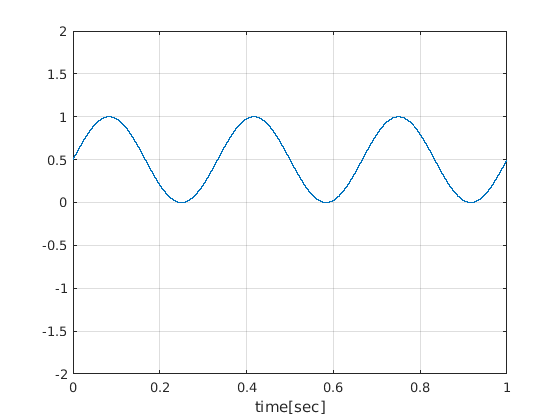
\includegraphics[width=11cm]{sine01.png}
 	\caption[sine 0 to 1]
 	{Sine with a range of 0-1. Obtained by taking a sine wave, adding 1 and dividing by two afterwards.}
 	\label{fig:sine01}
 \end{figure} 

Using what we got now in figure \ref{fig:sine01}, we can just multiply by 10, easy! Beware that there are always multiple solutions to this kind of a problem. Try to find another one for the problem above!

\begin{question}
Let's take a sine wave that has it's minimum at 2 and it's maximum at 5. What do we have to do to get it into a -1 to 1 range?
\end{question}
\begin{Answer}
We could subtract 1.5 to center the wave around zero first. Afterwardsm we take care of the amplitude by multiplying by $\frac{2}{3}$ (since the initial wave has a peak-to-peak amplitude of three and we want a peak-to-peak amplitude of 2)
\end{Answer}



\section{What's DC-Offset?}

What we did above by adding a constant value to a signal can be called adding DC-offset (``Gleichspannungsversatz''), DC-Bias or a DC component. These are different words for the same thing.\\
DC-offset can also be encountered in signals we recorded (caused by old or broken equipment mainly). But we have seen that we can also generate DC-offset.


\section{What's an Impulse?}

\section{How to describe audio mathematically}



\subsection{signals}

\subsection{systems}

% \addsec{Was passiert in Epro und wofuer brauche ich es?}

